\documentclass{beamer}
\mode<presentation>
{
  \usetheme{default}      % or try Darmstadt, Madrid, Warsaw, ...
  \usecolortheme{default} % or try albatross, beaver, crane, ...
  \usefonttheme{default}  % or try serif, structurebold, ...
  \setbeamertemplate{navigation symbols}{}
  \setbeamertemplate{caption}[numbered]
} 
\setbeamertemplate{footline}[frame number]

\usepackage[english]{babel}
\usepackage[utf8x]{inputenc}
\usepackage[round]{natbib}
\usepackage{gensymb}
\bibliographystyle{apalike}

% make bibliography entries smaller
\renewcommand\bibfont{\scriptsize}
% If you have more than one page of references, you want to tell beamer
% to put the continuation section label from the second slide onwards
\setbeamertemplate{frametitle continuation}[from second]
% Now get rid of all the colours
\setbeamercolor*{bibliography entry title}{fg=black}
\setbeamercolor*{bibliography entry author}{fg=black}
\setbeamercolor*{bibliography entry location}{fg=black}
\setbeamercolor*{bibliography entry note}{fg=black}
% and kill the abominable icon
\setbeamertemplate{bibliography item}{}

\title{Measurements of turbulence in Katabatic Winds on a steep slope}
%\author{Claudio Pierard}
\author[Your Name]{Claudio Pierard\\{\small Supervised by: Jean-Emmanuel Sicart}}
\institute{Master 1 Applied Mechanics\\ 
Universit\'e Grenoble Alpes \\
Institut des G\'eosciences de l'Environnement}
\date{23/01/2019}
\titlegraphic{
\includegraphics[height=1cm]{logo_UGA.png}}
\begin{document}

\begin{frame}
  \titlepage
\end{frame}

% Uncomment these lines for an automatically generated outline.
%\begin{frame}{Outline}
%  \tableofcontents
%\end{frame}

\section{Introduction}

%%%%%% 2 %%%%%%

\begin{frame}{Aim of study}

\begin{itemize}
\item Execute measurements of katabatic wind on a steep slope.
\item Measure velocity, temperature and radiation a long a vertical column.
\item Analyse the structure and characteristics of katabatic winds.
\end{itemize}

\begin{block}{Relevance}
\begin{itemize}
    \item Important role in local weather and pollution in mountainous regions.
    \item Not well parameterised in mesoscale models.
    \item Few field case studies on katabatic winds on steep slopes.
\end{itemize}
\end{block}

Based on the previous studies done by \cite{jakob}, \cite{claudine} and \cite{alban}.

\end{frame}

%%%%%% 3 %%%%%%

\section{Theory}

\begin{frame}{Boundary layer}
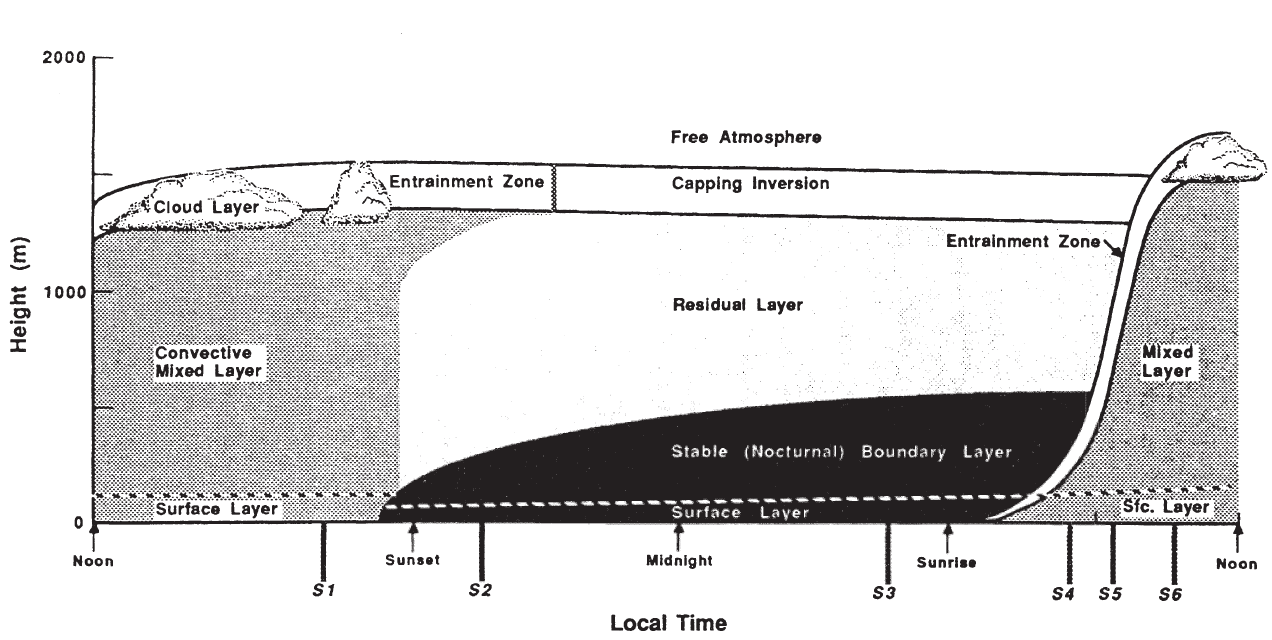
\includegraphics[width=1\textwidth]{abl_stull.png}

\hfill {\tiny \cite{stull2012introduction}}
\end{frame}

%%%%%% 4 %%%%%%

\begin{frame}{Katabatic wind}

\begin{columns}
\column{0.3\textwidth}
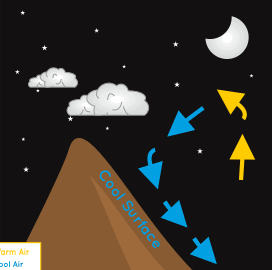
\includegraphics[width=1\textwidth]{kata.png}
\column{0.7\textwidth}
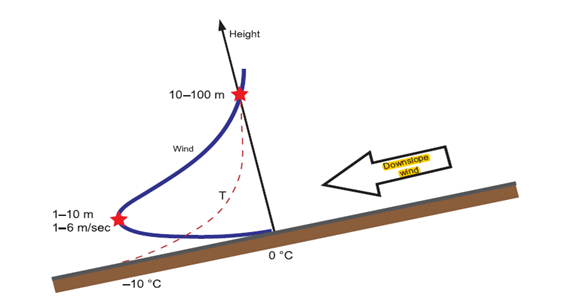
\includegraphics[width=1\textwidth]{katabatic.png}
\end{columns}

\hfill {\tiny \cite{poulos2008observational}}
\end{frame}

%%%%%% 5 %%%%%%
\addtobeamertemplate{block begin}{\vspace*{-3pt}}{}
\addtobeamertemplate{block end}{}{\vspace*{-3pt}}

\begin{frame}{Concepts}

\begin{block}{Turbulence Kinetic Energy (TKE)}
\begin{equation}
    e = \frac{1}{2} \big(\overline{u'^2} + \overline{v'^2} + \overline{w'^2}\big). 
    \label{eq:tke}
\end{equation}
\end{block}

\begin{block}{Covariance}
\begin{equation}
    \text{covar}(A,B) = \frac{1}{N}\sum_{i=0}^{N-1} a_i' b_i'= \overline{a'b'}.
\end{equation}
\end{block}

\begin{block}{Sensible heat flux}
\begin{equation}
    H = \rho \ C_p \ \overline{w'\theta'},
\end{equation}
\end{block}

\begin{block}{Momentum flux}
\begin{equation}
    F = \rho \ \overline{u'w'}, 
\end{equation}
\end{block}

\end{frame}

%%%%%% 6 %%%%%%

\section{Methodology}

\begin{frame}{Observational site \& field work}

\begin{columns}
\column{0.5\textwidth}
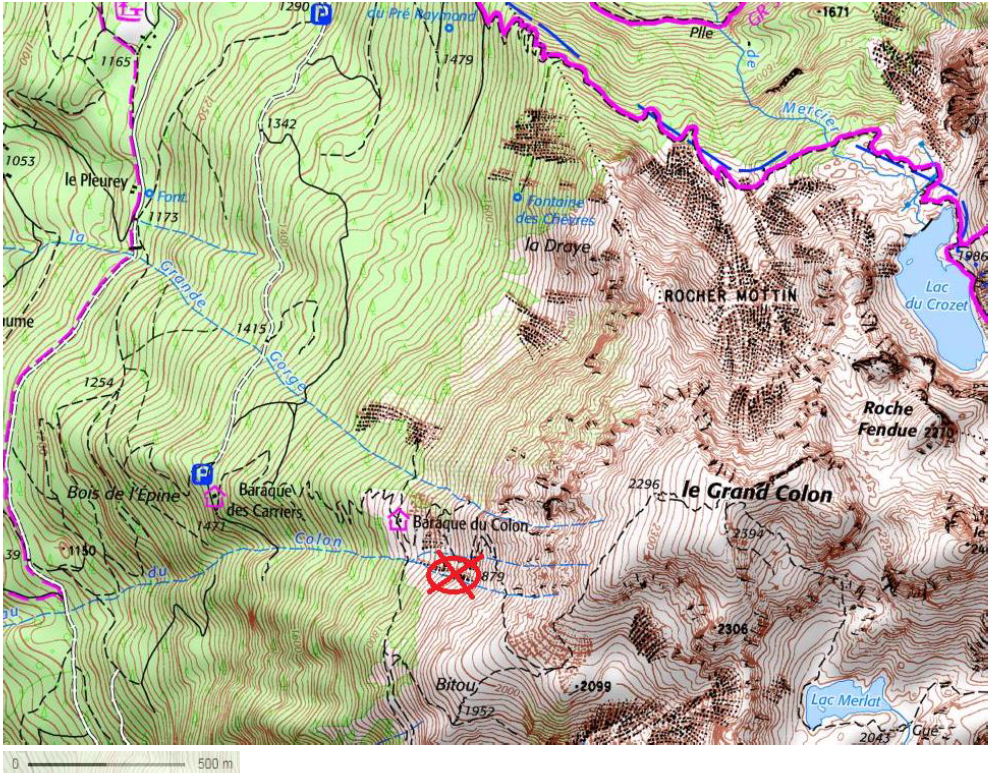
\includegraphics[width=1.1\textwidth]{grand_colon_jakob.png}
\column{0.5\textwidth}
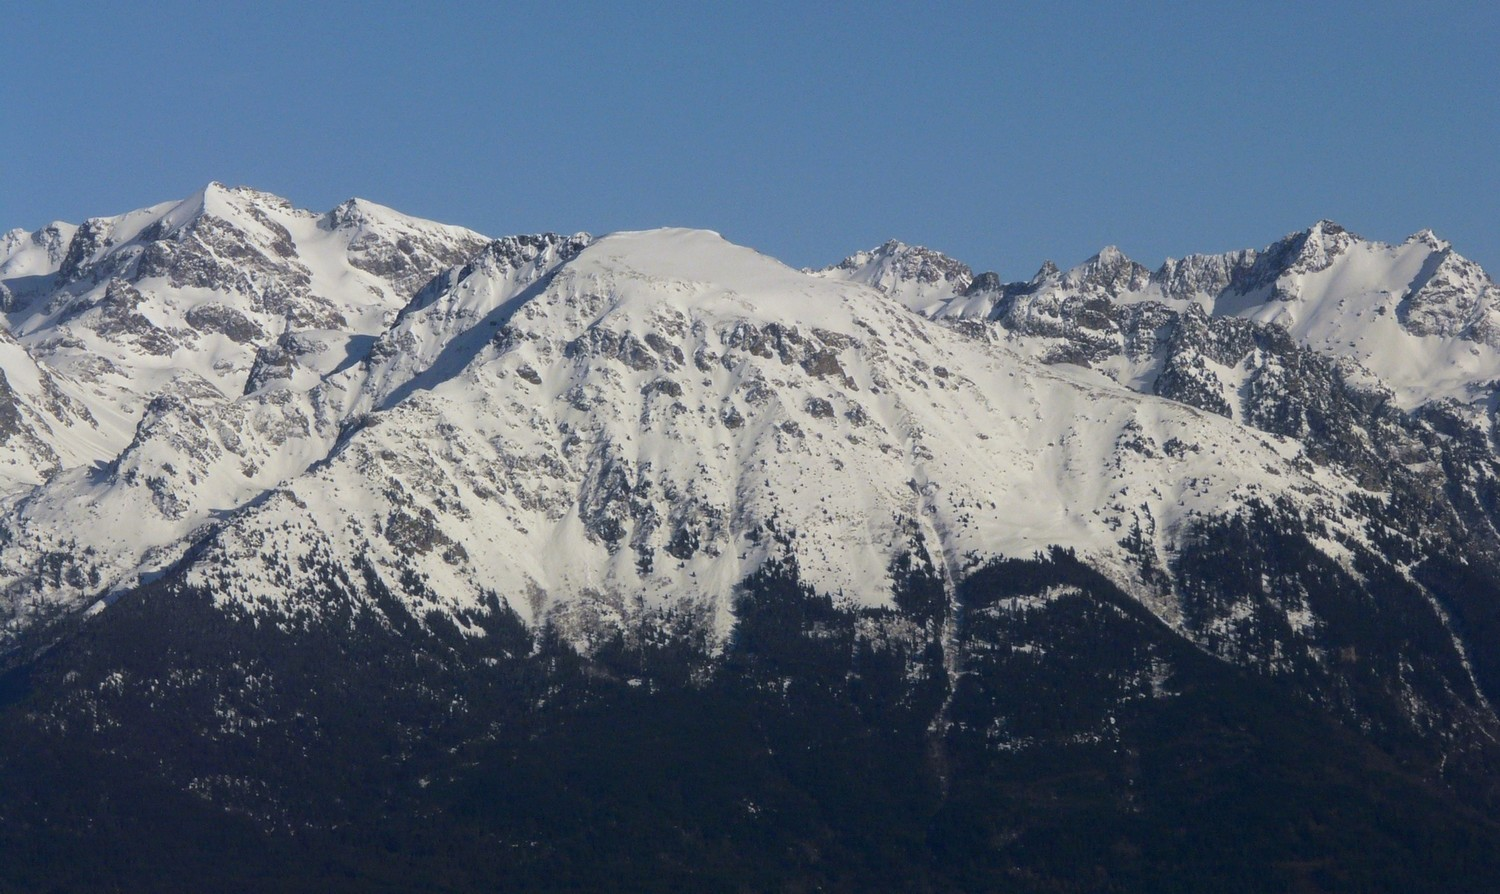
\includegraphics[width=1\textwidth]{gc.jpg}
\end{columns}

\begin{itemize}
    \item 1770 m above sea level.
    \item Slope of $21\degree$.
    \item In winter.
    \item Anticyclonic conditions: clear sky, cold nights and weak winds.
\end{itemize}
\end{frame}

%%%%%% 7 %%%%%%

\begin{frame}{Instrumentation}

\begin{columns}
\column{0.5\textwidth}
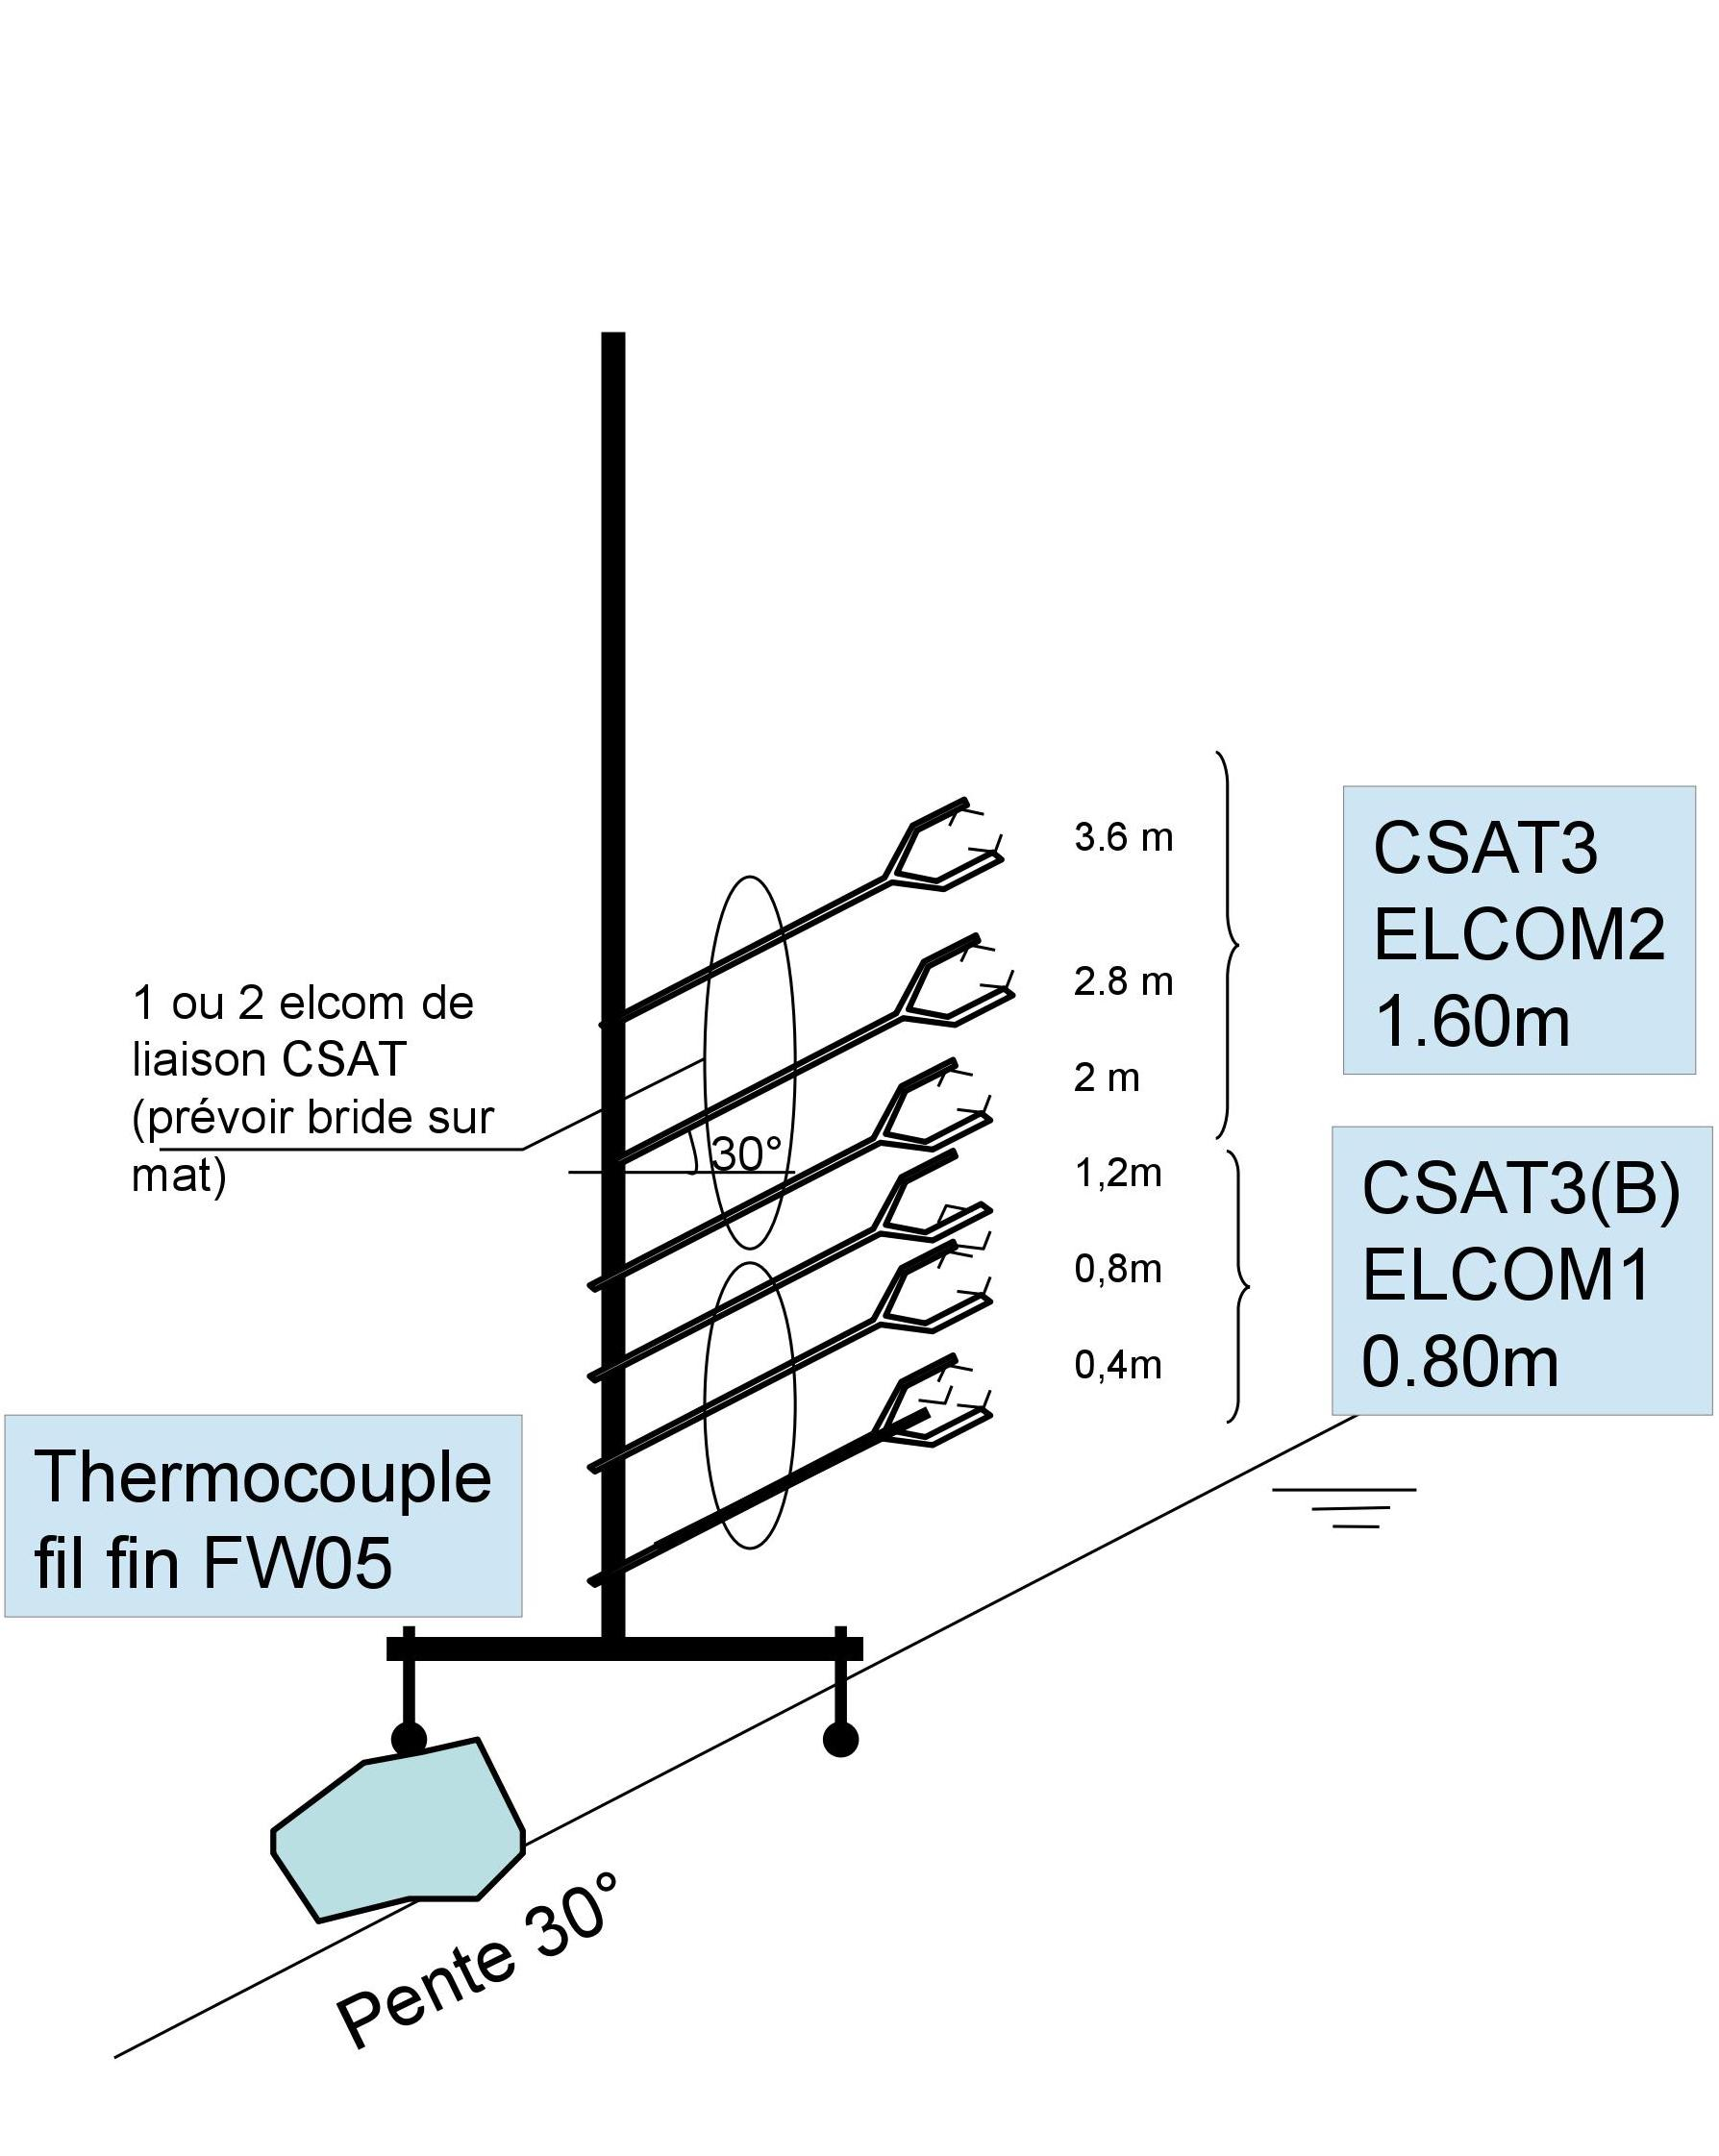
\includegraphics[width=1.1\textwidth]{0001.jpg}
\column{0.5\textwidth}
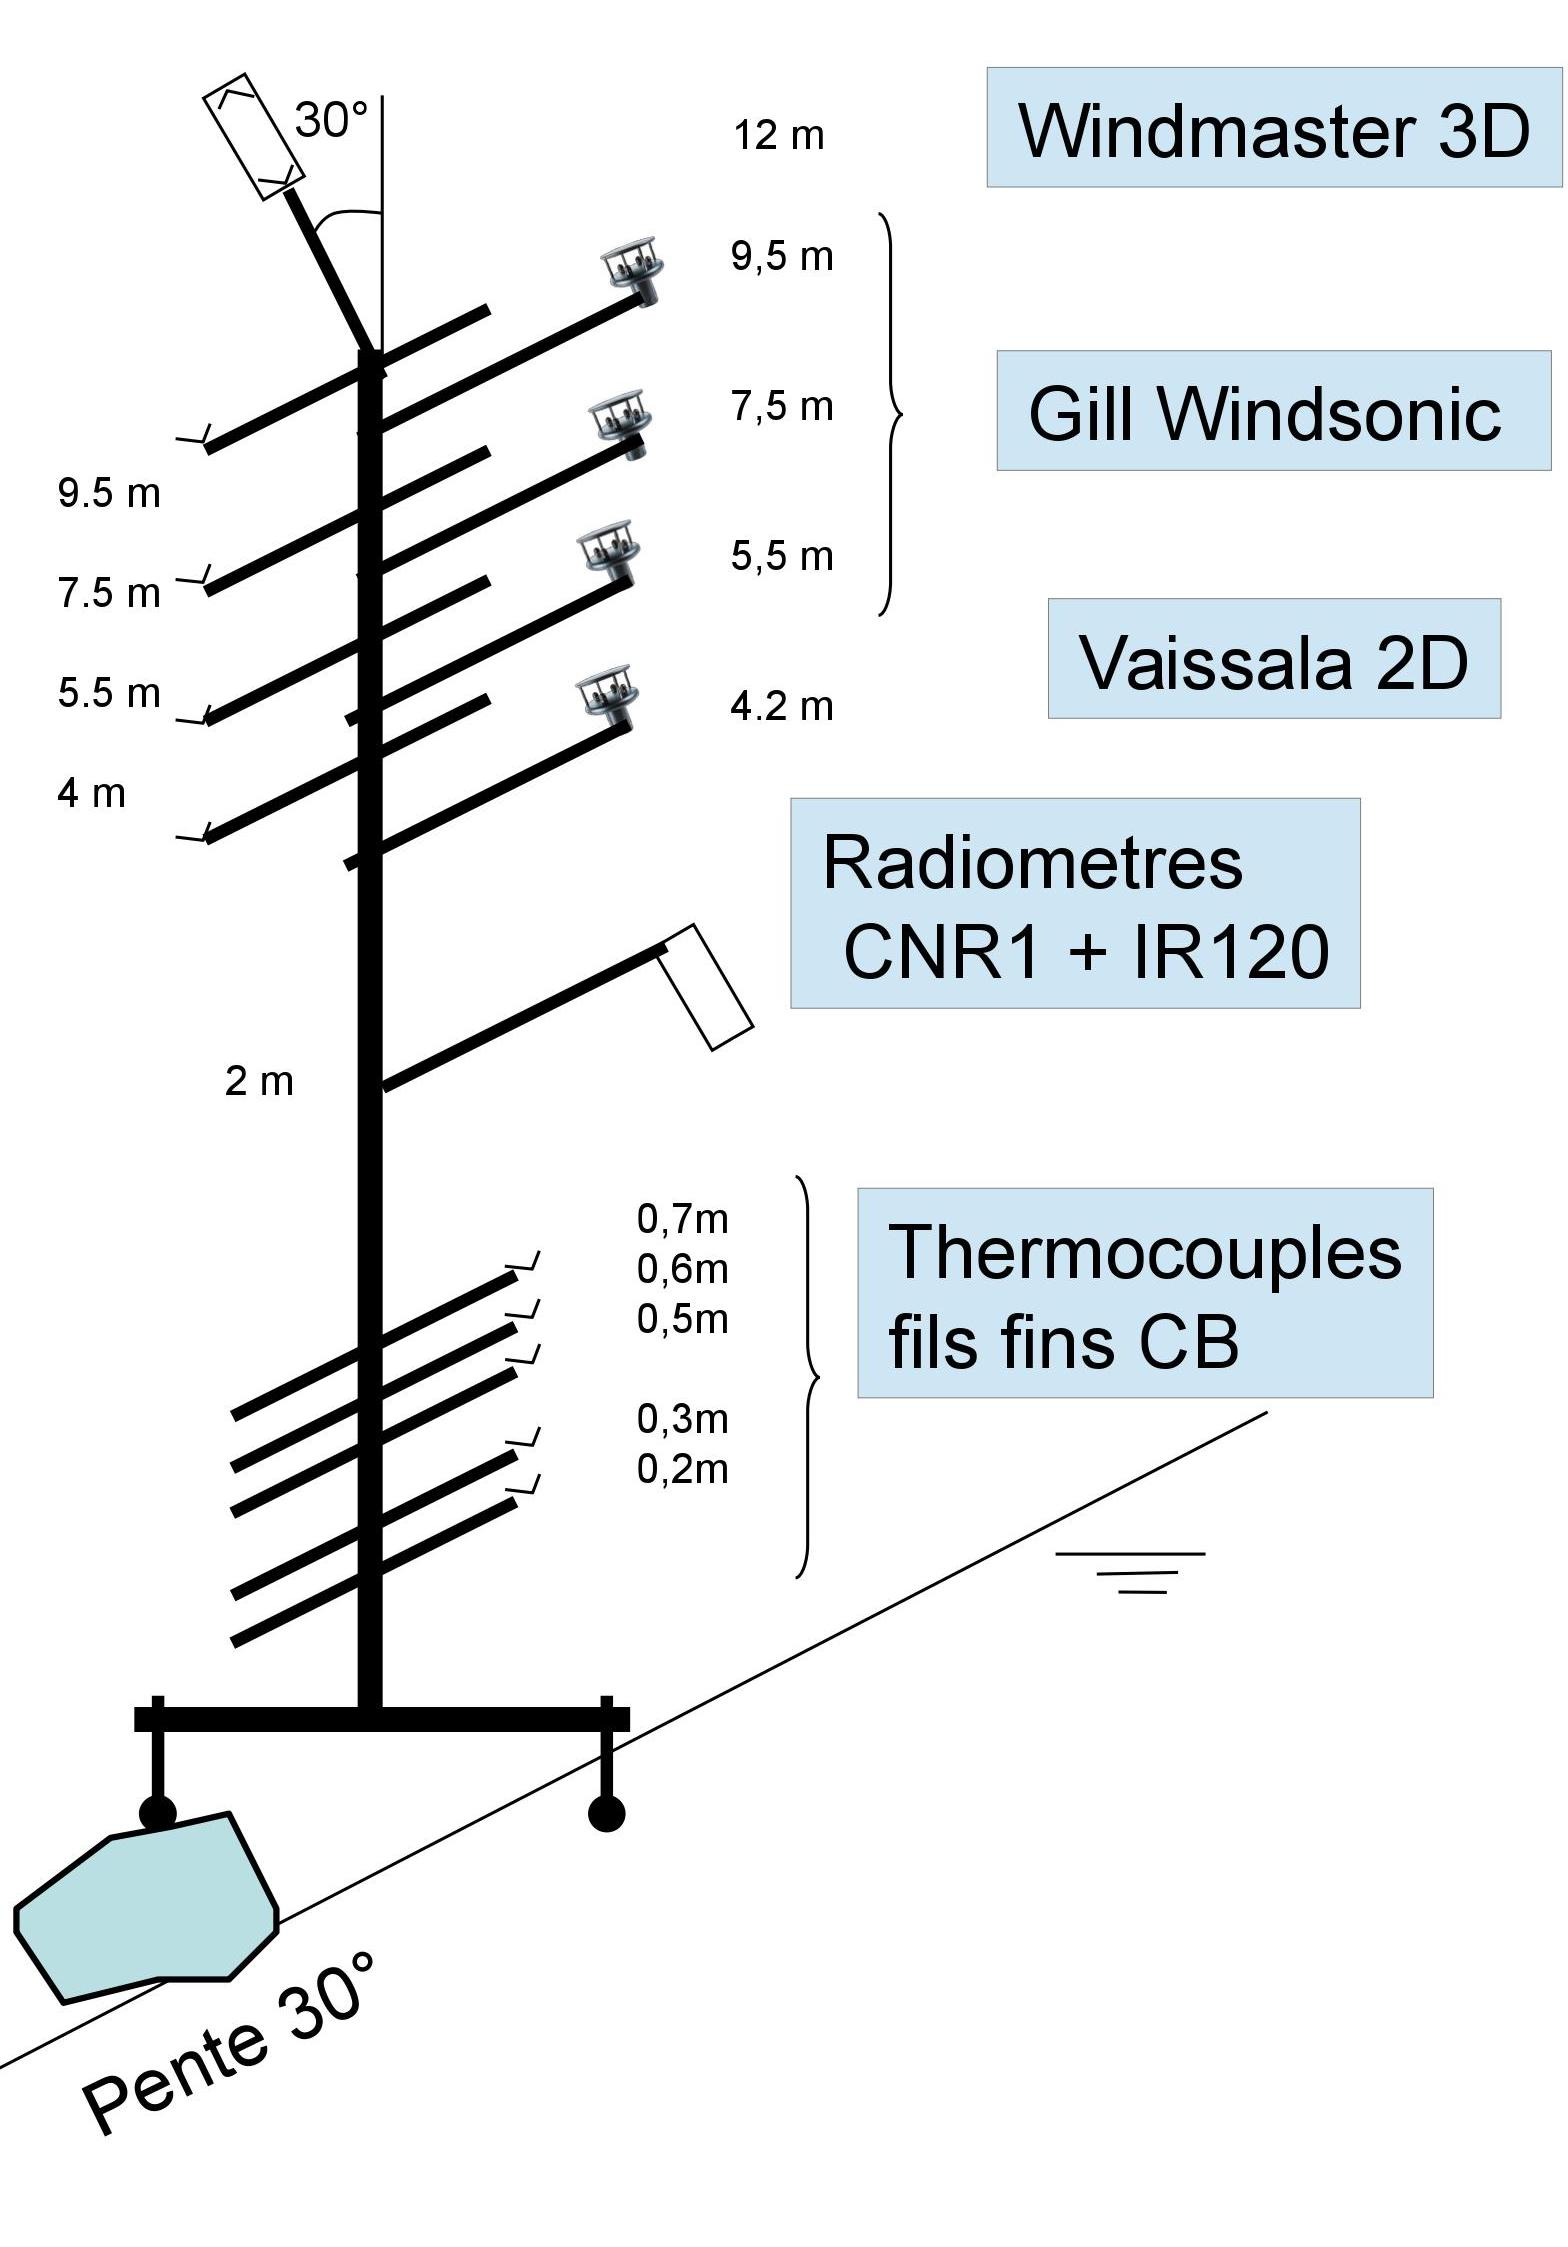
\includegraphics[width=1.1\textwidth]{0002.jpg}
\end{columns}

\end{frame}

%%%%%% 8 %%%%%%

\section{Timetable}

\begin{frame}{Workflow \& timetable}

\begin{itemize}
    \item Look for anticyclonic periods.
    \item Compute mean profiles and fluctuations of velocity, temperature and radiation, using EddyPro.
    \item Compute eddy fluxes.
\item Compute the TKE on different height levels 
\end{itemize}

\begin{table}[ht!]
\scriptsize 
%\centering
\begin{center}
\begin{tabular}{|c|c|p{6cm}|}
\hline
  & \textbf{Working days} & \textbf{Activity} \\
\hline
January & 1 & Field Work. Working on theory and foundations of the research.\\
\hline
February & 7 & Field Work. Analysis of the data, start to analyse 2015 data to get familiar with EddyPro.\\
\hline
March & 4 & Analysis of the data gathered during the field work.\\
\hline
April & 7 & Writing and analysing the data gathered.\\
\hline
May & 12 & Plotting the results and final analysis of the data sets. Working in the final report and oral presentation.\\
\hline
\end{tabular}

\label{table:schedule}
\end{center}
\end{table}


\end{frame}

%%%%%% 9 %%%%%%

\begin{frame}[allowframebreaks]{References}%[allowframebreaks] in case more than 1 slide needed
    \footnotesize
    \bibliographystyle{plainnat}
    \nocite{*}
    \bibliography{biblio}
    
\end{frame}

\end{document}
